% this file is called up by thesis.tex
% content in this file will be fed into the main document
\chapter{Fulguraciones solares}
% top level followed by section, subsection

Las fulguraciones solares (o llamaradas) son explosiones intensas en el Sol que viene de la liberación de la energía magnética asociada con las manchas solares. La radiación nociva de una llamarada no puede pasar a través de la atmósfera de la Tierra para afectar físicamente a los seres humanos a nivel de tierra. Aunque, cuando es suficientemente intensa,  puede afectar la ionosfera de la Tierra e interferir con nuestros sistemas de comunicaciones, como la radio y el GPS, y también perturbar la electrónica de satélites.\\


Debido la intensidad de emisión en rayos X, las fulguraciones solares se clasifican en A, B, C, M y X. Cada letra representa un aumento de 10 veces en la producción de energía\cite{nasa}. Así que una X es diez veces una M y 100 veces una C. En las figuras \ref{classM} y \ref{classX} se muestran dos clases de fulguraciones solares.\\

\begin{figure}[H]
\begin{minipage}{0.6\textwidth}
\begin{center}
\includegraphics[scale=0.05]{Apendice1/figs/claseM.jpg}
\footnote{\url{https://www.nasa.gov/content/goddard/nasa-releases-images-of-1st-notable-solar-flare-of-2015}} 
\end{center}
\end{minipage}
\hspace{0.1cm}
\begin{minipage}{0.4\textwidth}
\caption[Fulguración solar de clase M, 12 de enero de 2015]{El Sol emitió una fulguración solar de clase M, alcanzando su punto máximo a las 11:24 p.m. el 12 de enero de 2015. El Observatorio de Dinámica Solar de la NASA, que observa el sol constantemente, capturó una imagen del evento.}
\label{classM}
\end{minipage}
\end{figure}

Se recomienda ver las fotos y animaciones de las fulguraciones solares en la pestaña de galerías que se encuentra accediendo al enlace de cada imagen.

\begin{figure}[H]
  \centering
    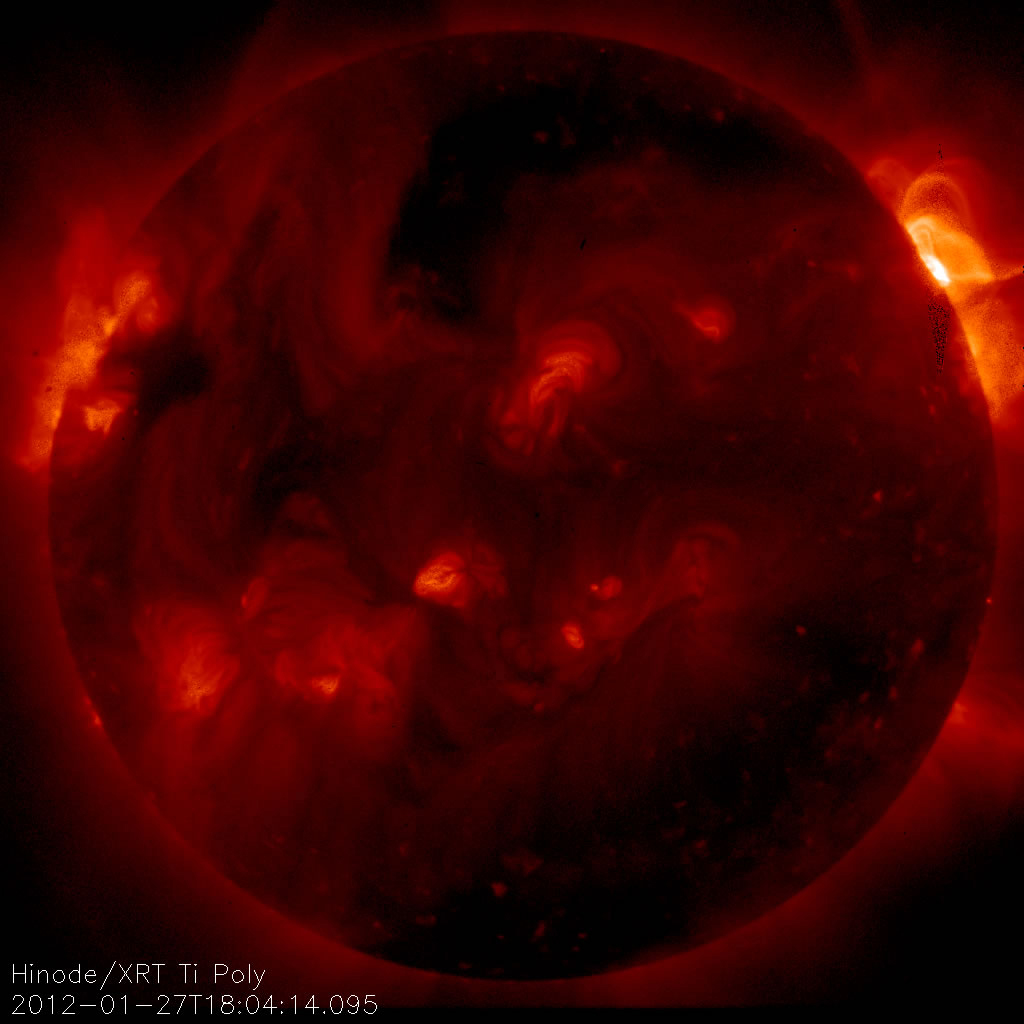
\includegraphics[scale=0.3]{Apendice1/figs/claseX.jpg}      %Ruta completa de la imagen, porque se compila desde el archivo tesis.tex
  \caption[Fulguración solar de clase X, 27 de enero de 2012]{El 27 de enero de 2012, estalló una fulguración intensa de clase X. Las fulguraciones de clase X son las explosiones más intensas. Aquí se ve una imagen de la llamarada capturada por el telescopio de rayos X en Hinode. Esta imagen muestra una emisión de plasma calentado a más de ocho millones de grados durante el proceso de liberación de energía de la llamarada. Imagen tomada de \url{https://www.nasa.gov/multimedia/imagegallery/image_feature_2169.html}}            %Pie de imagen
  \label{classX}                            %nombre de referencia
\end{figure}


\begin{figure}[H]
  \centering
    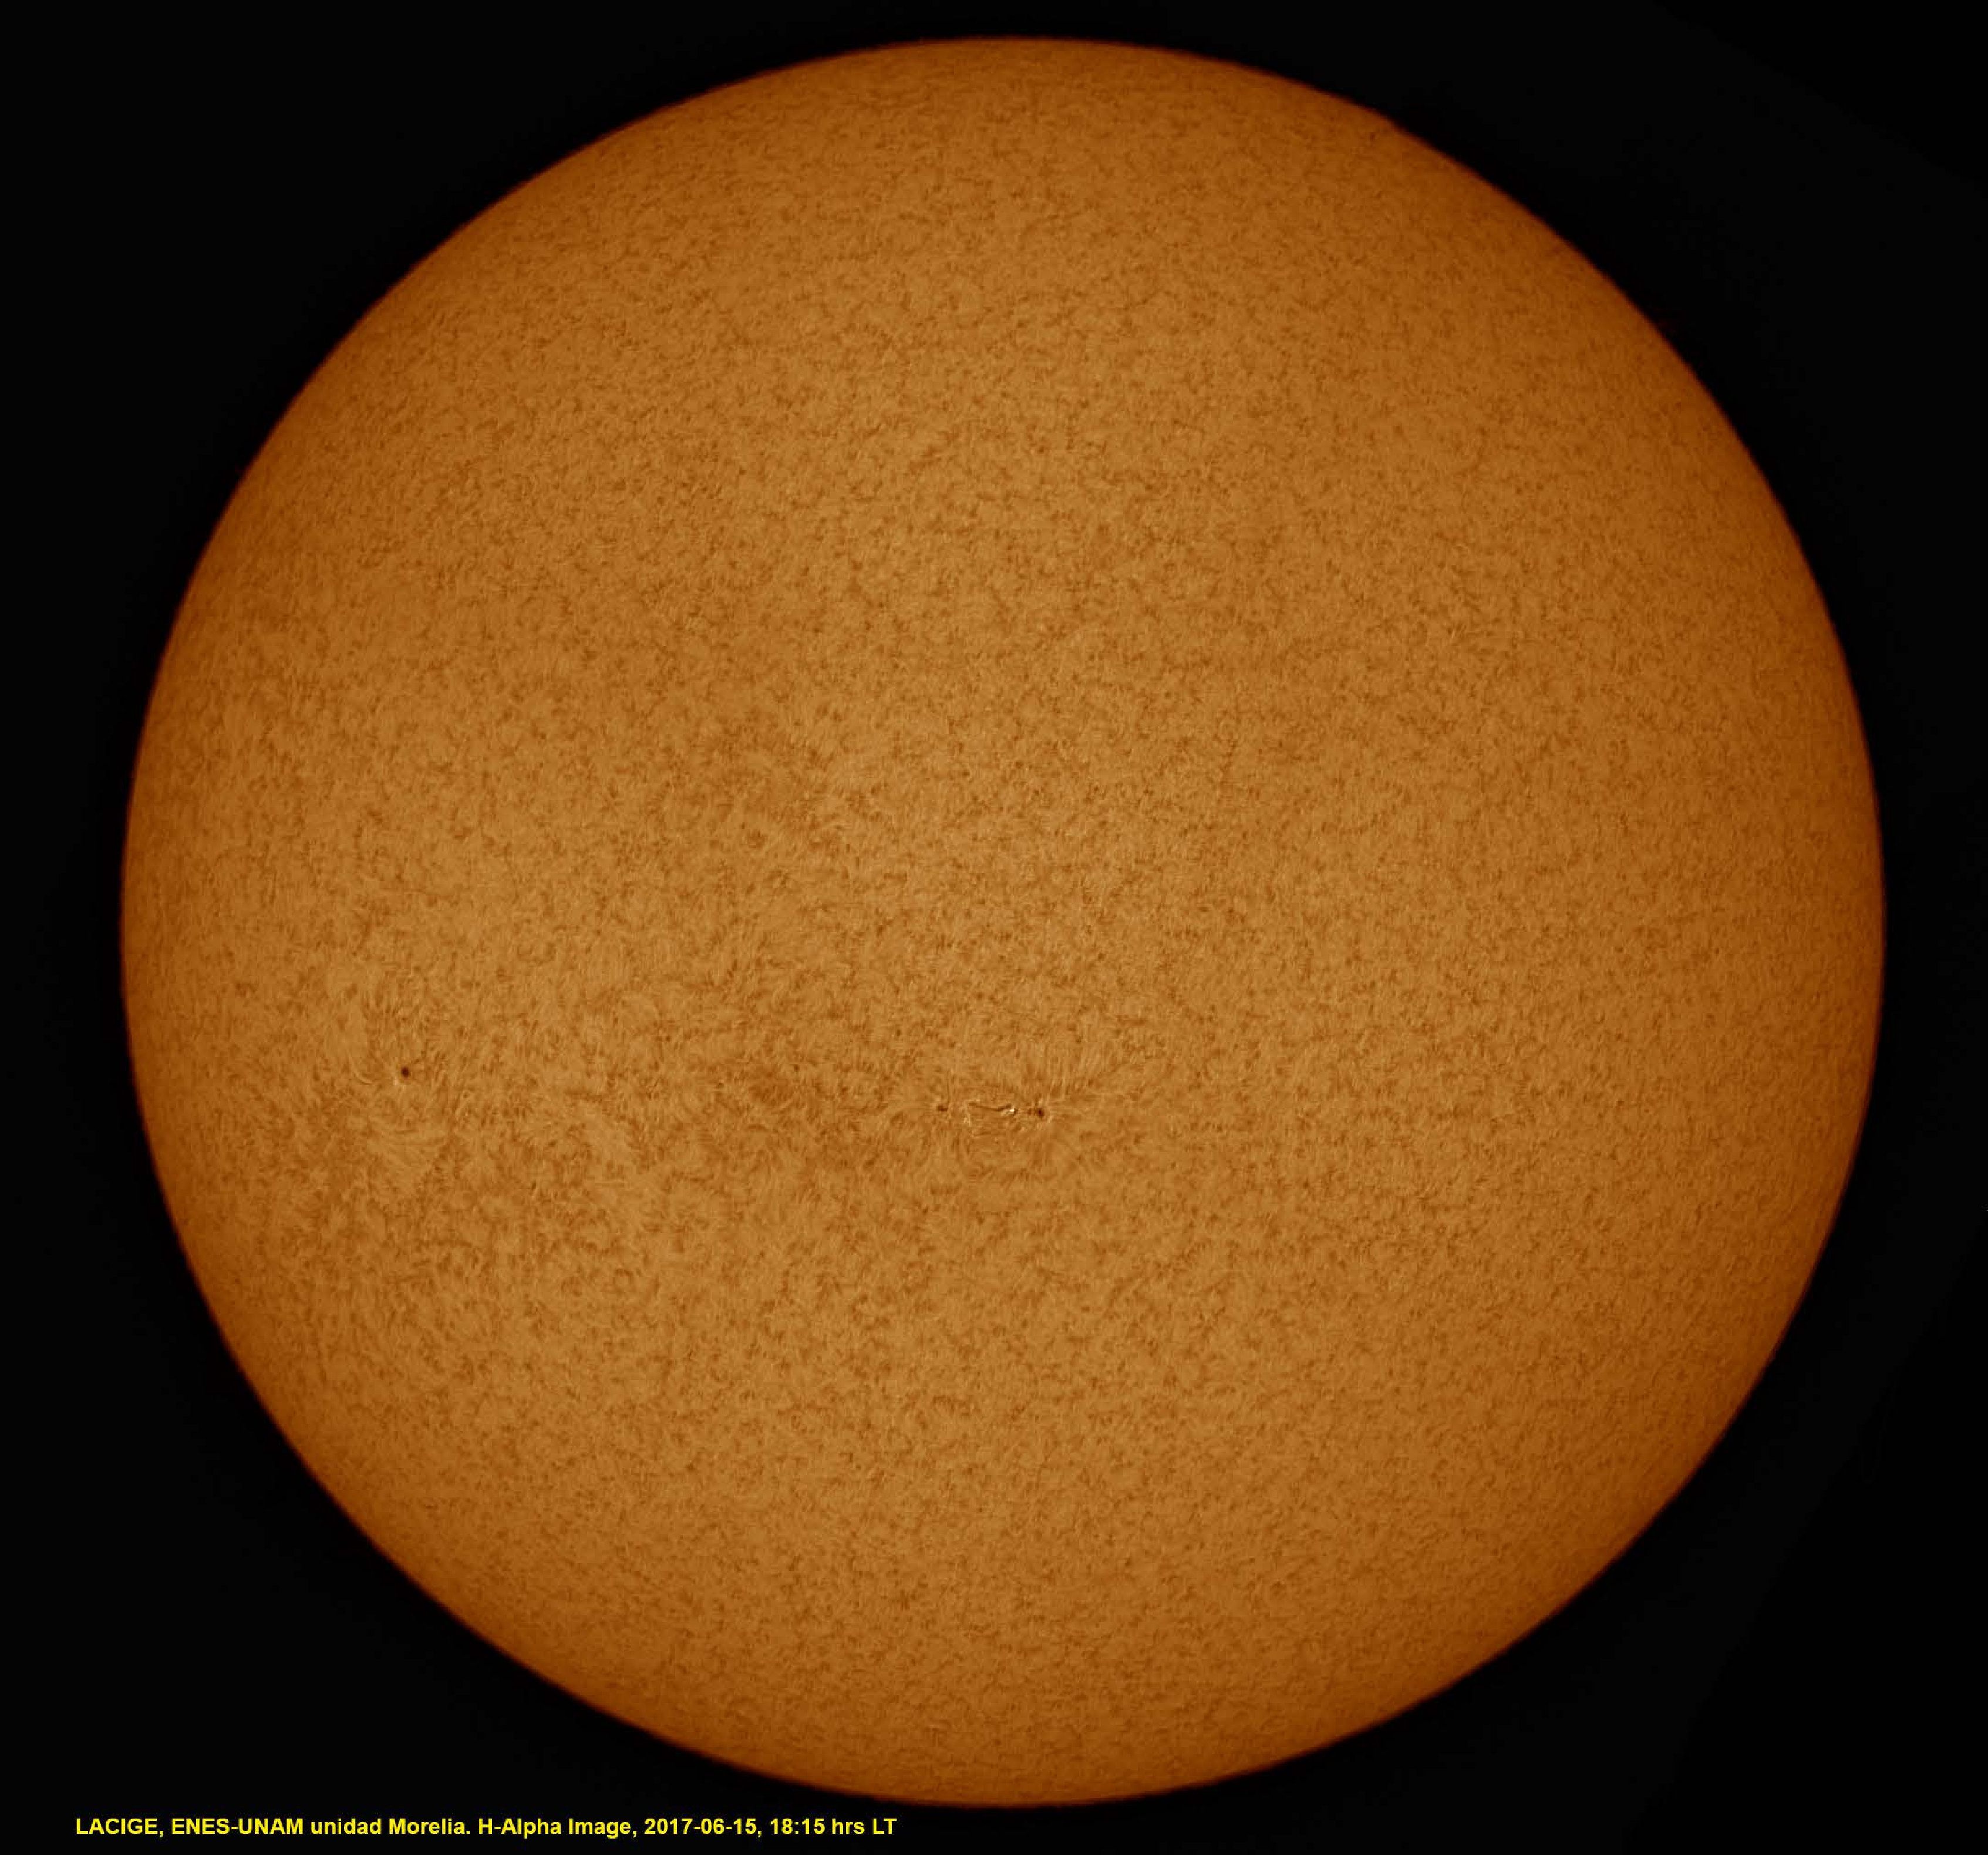
\includegraphics[scale=0.2]{Apendice1/figs/sol_compuesta.pdf}      %Ruta completa de la imagen, porque se compila desde el archivo tesis.tex
  \caption[El Sol con baja actividad]{Se muestra la imagen del Sol en el mínimo de actividad, nótese las diferencias con las figuras \ref{classM} y \ref{classX}. Es una imagen en el óptico (H-Alfa), que muestra la fotósfera solar, tomada por LACIGE, ENES-UNAM unidad Morelia.}            %Pie de imagen
  \label{minima_act}                            %nombre de referencia
\end{figure}


